\section{L9: Hash}

Hash 是一種 compression function。長的 input 經過 hash 之後會變成短的 ouput。 \\
Hash 也被稱為 fingerprint / hash value / digest。

因為是壓縮,所以會存在一些碰撞 (collision)。 \\
Collision: a pair of distinct items \(x, x'\) for which Hash(x) = Hash(x')。


\subsection{Syntax}

\begin{definition}
	A hash function (with output length \(l(n)\)) is a pair of PPT algorithm \((\Gen, \H)\)
	\begin{myItemize}
		\item \(\Gen\): takes a security parameter \(1^n\) and outputs a key \(s\).
		\item \(\H\): takes input as a key \(s\) and a string \(x \in \{0, 1\}^\ast\), and outputs a string \(\H^s(x) \in \{0, 1\}^{l(n)}\).
	\end{myItemize}
\end{definition}

If \(x \in \{0, 1\}^{l'(n)}\) and \(l'(n) > l(n)\), then we say it's a fixed-length input hash.

\vspace{1cm}

\begin{definition}[Collision resistant]
	A hash function \(\Pi = (\Gen, \H)\) is collision resistant if \(\forall\) PPT adversaries \(A\), there is a negligible function \(\negl\) such that
	\[\Pr[\HashColl_{A, \Pi}(n) = 1] \leq \negl(n)\]
\end{definition}

\(\HashColl_{A, \Pi}(n)\) 的 scenario 如下:
\begin{center}
	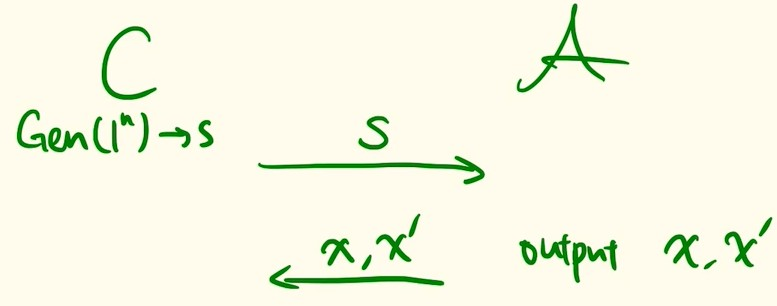
\includegraphics[width=0.4\textwidth, keepaspectratio]{Hash-coll_scenario.jpg}
\end{center}
首先 challenger \(C\) 會先產生一個 key \(s\) 給 adversary \(A\)。\(A\) 可以通過自己的計算,試圖猜出一個 pair \((x, x')\),再傳給 \(C\)。若 \(\H^s(x) = H^s(x')\) 且 \(x \neq x'\),則 output 1,也就是 \(\HashColl_{A, \Pi}(n) = 1\)。

\paragraph{Preimage resistant (one-wayness)}

Adversary 會拿到一個 key \(s\)(下圖省略)和一個 hash function \(\H\) 的 output \(y\),並且當 adversary 給出 \(x = \H^{-1}(y)\) 時,視為破解成功。
\begin{center}
	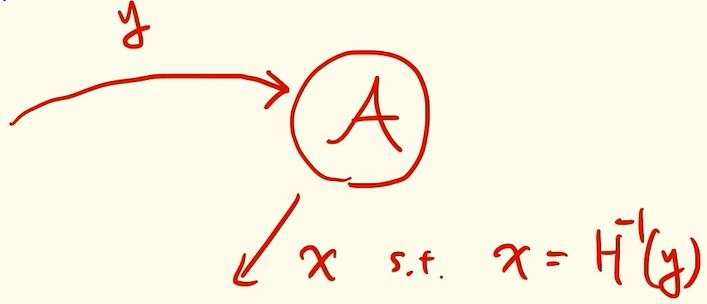
\includegraphics[width=0.5\textwidth, keepaspectratio]{preimage_resistant.jpg}
\end{center}

\paragraph{Second-preimage resistant}

Adversary 會拿到一個 key \(s\)(下圖省略)和一對 value \textemdash{} hash function \(\H\) 的 input \(x\) 和 output \(y = H(x)\),並且當 adversary 給出 \(x' \neq x\) 且 \( \H(x') = \H(x)\) 時,視為破解成功。
\begin{center}
	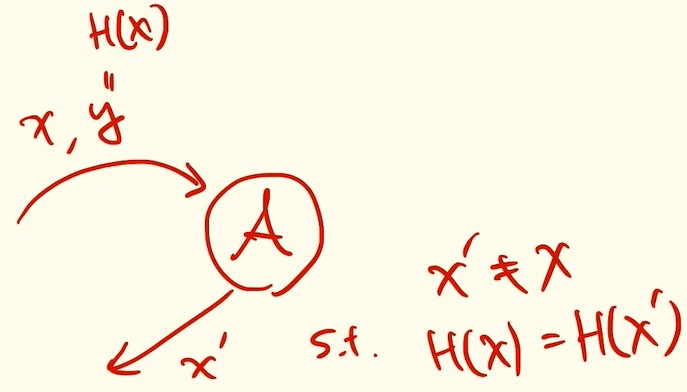
\includegraphics[width=0.5\textwidth, keepaspectratio]{second-preimage_resistant.jpg}
\end{center}

若要以上述情況作為 security 的定義,則兩者成功的機率都是要 \(\leq \negl\)。

\subparagraph{Quiz}

Compare the security notions of hash function. 比較各種 hash function 的安全定義的難易程度(易、難、無法比較) \\
(Ex:Second-preimage resistant is harder than collision resistant.)


\subsection{SIS}


\paragraph{Short Integer Solution (SIS) Problem}

\(\mathbb{Z}_q^n\): n-dimensional vectors modulo \(q\) (e.g. \(q \approx\ n^3\))

Goal: find non-trivial small (ex: \(\{0, 1\}\)) \(z_1, z_2, \ldots, z_m \in \mathbb{Z}\) such that
\[
	z_1 \begin{bmatrix} a_{11} \\ a_{12} \\ \vdots \\ a_{13} \end{bmatrix}
	+ z_2 \begin{bmatrix} a_{21} \\ a_{22} \\ \vdots \\ a_{23} \end{bmatrix} 
	+ z_m \begin{bmatrix} a_{m1} \\ a_{m2} \\ \vdots \\ a_{m3} \end{bmatrix}
	= \begin{bmatrix} 0 \\ 0 \\ \vdots \\ 0 \end{bmatrix}
	\in \mathbb{Z}_q^n
\]

Remark:
\begin{myItemize}
	\item \(z_1, z_2, \ldots, z_m = 0 \quad \Rightarrow \quad\) ``trival"
	\item \(z_1, z_2, \ldots, z_m \not\in \{0, 1\} \quad \Rightarrow \quad\) ``easy"
\end{myItemize}


\paragraph{SIS-based Hash Function}

Rewrite the forementioned definition of SIS problem.

\(\mathbb{Z}_q^n\): n-dimensional vectors modulo \(q\) (e.g. \(q \approx\ n^3\))

Goal: find non-trivial small (ex: \(\{0, 1\}\)) \(z_1, z_2, \ldots, z_m \in \mathbb{Z}\) such that
\[
	\mathbf{A} \mathbf{z} = 
	\begin{bmatrix}
		\phantom{a_11} & \phantom{a_{12}} & \phantom{a_{13}} & \phantom{a_{14}} \\
		\phantom{a_11} & \phantom{a_{12}} & \phantom{a_{13}} & \phantom{a_{14}} \\
		a_1 & a_2 & \ldots & a_m \\
		\phantom{a_11} & \phantom{a_{12}} & \phantom{a_{13}} & \phantom{a_{14}} \\
		\phantom{a_11} & \phantom{a_{12}} & \phantom{a_{13}} & \phantom{a_{14}} \\
	\end{bmatrix}
	\begin{bmatrix}
		z_1 \\ z_2 \\ \vdots \\ z_m
	\end{bmatrix}
	= \mathbf{0}
	\in \mathbb{Z}_q^n
\]

\subparagraph{Construction of Hash}

Set \(m > n \log q\) (for compression). \\
Define \(f_{\mathbf{A}}: \{0, 1\}^m \rightarrow \mathbb{Z}_q^n\) as \(f_{\mathbf{A}}(x) = \mathbf{Ax}\) 

Collision: \(\mathbf{x}, \mathbf{x'} \in \{0, 1\}^m\) where \(\mathbf{x} \neq \mathbf{x'}\) and \(\mathbf{Ax} = \mathbf{Ax'}\)


\paragraph{Collision Resistant SIS-based Hash}

\begin{center}
	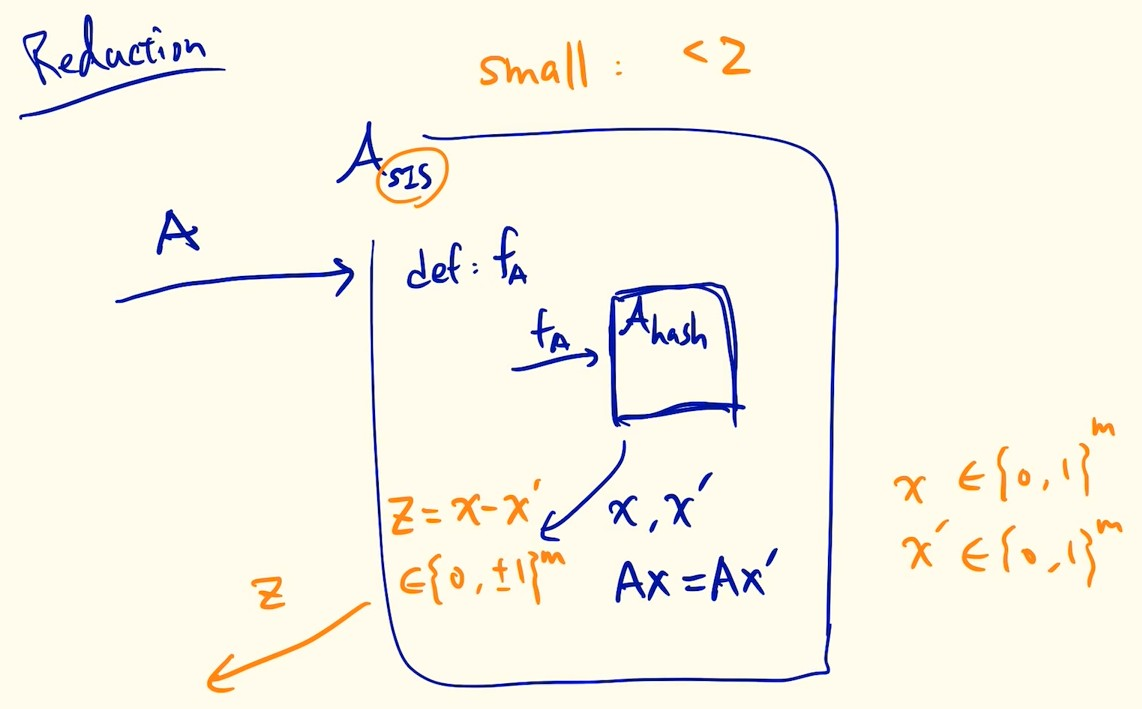
\includegraphics[width=0.7\textwidth, keepaspectratio]{SIS-based_hash_reduction.jpg}
\end{center}

\subparagraph{Quiz}

We do not formally write down the security proof, and only provide proof intuition.
\begin{enumerate}[label=(\roman*)]
	\item Please show the assumption (\(\Pr[success] \leq \negl\)), aka SIS, which is used in the proof.
	\item Please complete the proof with probability analysis.
\end{enumerate}


\subsection{Arbitrary-length Hash Function}

前面介紹的 SIS-based hash function 和現實中使用的 hash function 都是 fixed-length compression function。我們可以透過 Merkel-Damgard transformation 來做到 arbitrary-length hash function。

\paragraph{Merkle-Damgard Transformation}

和 CBC-MAC 的概念相似。

Let \((\Gen', \h)\) be a fixed input length hash. \(\h:\{0, 1\}^{2n} \rightarrow {0, 1}^n\) \\
Let \((\Gen, \H)\) be a fixed input length hash. \(\H:\{0, 1\}^\ast \rightarrow {0, 1}^n\)

Use \((\Gen, \h)\) to build \((\Gen, \H)\)
\begin{itemize}
	\item \(\Gen\): run \(\Gen'(1^n) \rightarrow s\) (key)
	\item \(\H\): on input \(s\) and a string \(x \in \{0, 1\}^\ast\) of length \(L\) where \(L < 2^n\).
		\begin{enumerate}[label=(\roman*)]
			\item Set \(B = \ceil{\frac{L}{n}}\) (\(B\): number of blocks) \\
				Pad \(x\) with \(0\)s, so length will be a multiple of n. \\
				Parse \(x\) to \(x_1, x_2, \ldots, x_B\), and set \(x_{B+1} = L\)
			\item Set \(z_0 = 0^n\) as IV
			\item For \(i = 1, 2, \ldots, B+1\), compute \(z_i = \h^s(z_{i-1} || x_i)\) \\
				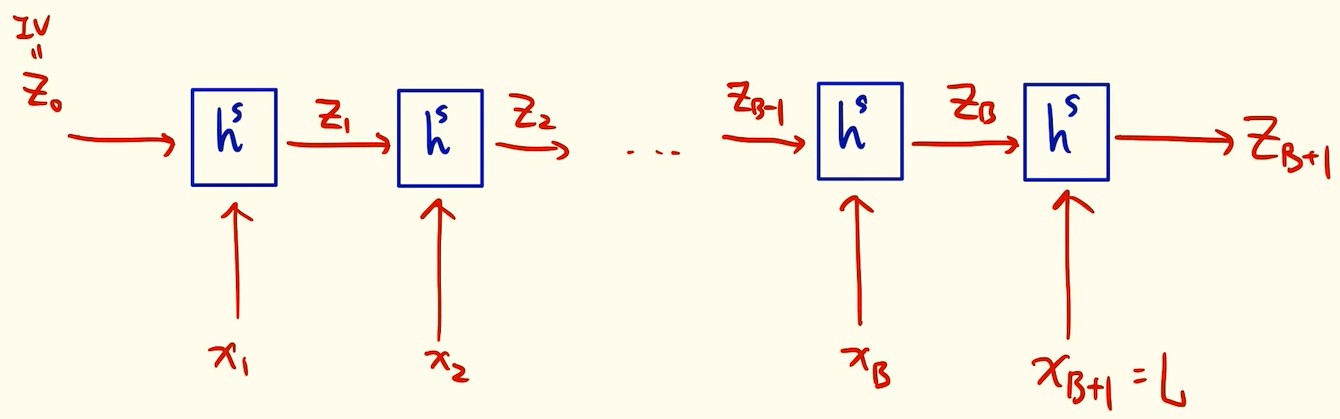
\includegraphics[width=\linewidth, keepaspectratio]{MD_transformation_step3.jpg}
			\item Output \(z_{B+1}\) as the hash value of \(x\).
		\end{enumerate}
\end{itemize}

\subparagraph{Quiz}

We found some cute trick in Merkle-Damgard transformation:
\begin{enumerate}[label=(\roman*)]
	\item The purpose of \(L\)? (Hint: related to collision)
	\item Suppose the fixed-length hash is \(h:{0, 1}^{n+1} \rightarrow {0, 1}^n\) \\
		How to build an arbitrary length has from the above?
\end{enumerate}


\paragraph{Security of Merkel-Damgard Transformation}

\begin{theorem}
	If \((\Gen', \h)\) is collision resistant, then \((\Gen, \h)\) is collision resistant.
\end{theorem}

\begin{myProof}
	For any \(s\), a collision in \(\H^s\) yields a collision \(h^s\). \\
	Assume two distinct strings \((x, x')\) of length \((L, L')\) such that \(\H^s(x) = \H^s(x')\).
	
	Let \(x_1, x_2, \ldots, x_B\) are the blocks of padded \(x\) and \(x_{B+1} = L\), \\
	and \(x'_1, x'_2, \ldots, x'_B\) are the blocks of padded \(x'\) and \(x_{B'+1} = L'\).
	
	\begin{enumerate}[label={Case \arabic*:}, leftmargin=50pt]
		\item \(L \neq L'\) \\
			In the last step of \(\H^s(x)\) (resp. \(\H^s(x')\)), \\
			\(z_{B+1} = \h^s(z_B || L)\) (resp. \(z'_{B'+1} = \h^s(z'_{B'} || L')\))
			
			Assume \(\H^s(x) = \H^s(x')\) \\
			\(\Rightarrow\) \quad \(h^s(z_B || L) = h^s(z'_{B'} || L')\)
			which is a collision in \(\h^s\)
		
		\item \(L = L'\) (implies \(B = B'\)) \\
			Let \(I_i \overset{\mathrm{def}}{=} z_{i-1} || x_i\). (\(i\)-th input of \(\h^s\)) (\(I'_i\), resp.) \\
			Set \(I_{B+2} \overset{\mathrm{def}}{=} z_{B+1}\).
			
			Assume \(\H^s(x) = \H^s(x')\). Let \(N\) be the largest index for \(I_N \neq I'_N\). \\
			Since \(|x| = |x'|\), but \(x \neq x'\), there must exist an \(i\) with \(x_i \neq x'_i\). \\
			\(I_{B+2} = z_{B+1} = \H^s(x) = \H^s(x') = z'_{B+1} = I'_{B+2}\) \\
			\(\Rightarrow\) \quad \(N \leq B+1\)
			\(\Rightarrow\) \quad \(I_{N+1} = I'_{N+1}\)
			
			For this \(N\), \(I_N, I'_N\) are collision in \(\h^s\).
	\end{enumerate}
\end{myProof}
